% Format:  Latex Orientation:  Portrait
% MASTERFILE
%
% Last change: <Thu, 2016/05/26 10:25:26 arwagner l00slwagner.desy.de>
%
\documentclass[presentation, 10pt]{beamer}
% use ``handout'' instead of ``presentation'' to create a 2 on 1 page
% handout version of the document

\mode<handout>{%
	\usepackage{pgf}
	\usepackage{pgfpages}
	\pgfpagesuselayout{2 on 1}[a4paper,border shrink=5mm]
}
\mode<presentation>{%
	\usetheme{DESY}
}
%% Setup for Beamer
\usepackage{xcolor}
\usepackage{hyperxmp}
% \usepackage[pdfa]{hyperref}
\usepackage{luatextra}
\usepackage{wasysym}
\usepackage{eurosym}
\usepackage{bookmark}
\usepackage{graphicx}
\usepackage{fontspec}
\setmainfont{Arial}
\usepackage[ngerman,english]{babel}
\usepackage{xspace}
\usepackage{tikz}

\tikzset{%
  every overlay node/.style={%
    %draw=black,fill=white,rounded corners,anchor=north west,
    draw=fzjlightblue,fill=fzjgray30,rounded corners,anchor=north west,
  },
}
% Usage:
% \tikzoverlay at (-1cm,-5cm) {content};
% or
% \tikzoverlay[text width=5cm] at (-1cm,-5cm) {content};
\def\tikzoverlay{%
   \tikz[baseline,overlay]\node[every overlay node]
}%


% General new commands an macros
\renewcommand{\emph}[1]{\structure{#1}}

\newcommand{\link}[2]{\href{#1}{~#2}}

\newcommand{\jointwo}{\textbf{JOIN$^2$}\xspace}

\newcommand{\BibTeX}{Bib\TeX}
\newcommand{\JabRef}{\link{http://jabref.sf.net}{JabRef}\xspace}
\newcommand{\Companion}[1]{\textit{\link{http://julib.fz-juelich.de/uhtbin/field-search-sort/001/PBYR/213964}{\LaTeX{} Companion}, #1}\xspace}
\newcommand{\pkg}[1]{\emph{\texttt{#1}}\xspace}

% general colour definitions
\newcommand{\smallgray}[1]{{\tiny\emph{#1}}}

\newcommand{\idR}{i.~d.~R.\xspace}
\newcommand{\va}{v.~a.\xspace}
\newcommand{\sa}{s.~a.\xspace}
\newcommand{\zB}{z.~B.\xspace}
\newcommand{\zT}{z.~T.\xspace}
\newcommand{\ggf}{ggf.\xspace}
\newcommand{\eg}{e.~g.\xspace}

\newcommand{\bs}[1]{\texttt{$\backslash$#1}}
\newcommand{\command}[2]{\texttt{\bs{#1}\{#2\}}}
% http://tex.stackexchange.com/questions/16447/beamer-top-aligning-columns-within-a-top-aligned-fram
\makeatletter
\newenvironment{topitemize}{%
   \setlength{\topsep}{0pt}
   \setlength{\partopsep}{0pt}
   \renewcommand*{\@listi}{\leftmargin\leftmargini \parsep\z@ \topsep\z@ \itemsep\z@}
   \let\@listI\@listi
   \itemize
}{\enditemize}
\makeatother


\title{DQM4HEP \\ Status and prospectives}
% subtitle is required for DESY beamer, set at least a space ~
\subtitle{CHEF 2017 - Lyon}

\author[R. Ete]{\underline{R. Ete}, A. Pingault}
\institute{DESY}
\date{\today}

\newenvironment{topitemize}{%
   \setlength{\topsep}{0pt}
   \setlength{\partopsep}{0pt}
   \renewcommand*{\@listi}{\leftmargin\leftmargini \parsep\z@ \topsep\z@ \itemsep\z@}
   \let\@listI\@listi
   \itemize
}{\enditemize}

\usepackage{makecell}

%---------------------------------------------------------------------

\begin{document}

\maketitle

%----------------------------------------------------------------------
\begin{frame}
  \frametitle{Summary}

  \begin{itemize}
    \item Introduction
    \item Framework presentation
    \item Experiments running with DQM4HEP
    \item EUDAQ / DQM4HEP interface
    \item Current status
    \item Ongoing and future working
  \end{itemize}
  
\end{frame}

%----------------------------------------------------------------------
\begin{frame}
  \frametitle{Introduction}
  \footnotesize
  DQM systems in HEP domain :
  \begin{itemize}
    \item Evaluate data quality and alert users of anomalies
    \item Yet developped for most of HEP experiments (i.e AMORE or CMSSW)
    \item Provide for online and offline analysis
    \begin{itemize}
      \item Automatic data quality tests, possibly with reference histograms
      \item Distributed system for online analysis (data collectors)
      \item Dedicated visualization interface (Qt, Web)
    \end{itemize}
  \end{itemize}
  ~\\
  \textbf{But ...} Based on experiment specific event format
  \begin{itemize}
    \item Not re-usable by other experiments
    \item Dulicated software
    \item Ad-hoc solution for test-beam setup monitoring
  \end{itemize}
  ~\\
  Development of a generic DQM software for any HEP experiment : \textbf{DQM4HEP}
\end{frame}



%----------------------------------------------------------------------
\begin{frame}
  \frametitle{DQM4HEP}
  \framesubtitle{Software overview}
  \footnotesize
  Key points : 
  \begin{itemize}
    \item Standalone plugin system (dynamic shared lib loading) 
    \item \textbf{Event data model/format + event streaming abstraction}
  \end{itemize}
  ~ \\
  More general features :
  \begin{itemize}
    \item Online analysis (API)
    \item Streaming tools for event read/write functions
    \item Distributed system (DIM)
    \item Data collectors : event and histogram collector servers
    \item Quality test tools : interface + many template
  \end{itemize}
\end{frame}


%----------------------------------------------------------------------
\begin{frame}
  \frametitle{DQM4HEP}
  \framesubtitle{Quality test API}
  \footnotesize
  \begin{block}{Monitor element}
    \begin{itemize}
      \item Wrap a ROOT TObject 
      \item Optional hold a ROOT TObject as reference
    \end{itemize}
  \end{block}
  \begin{block}{Quality test}
    \begin{itemize}
      \item Implement the logic a testing a monitor element
      \item Output a quality report (quality flag, success, etc)
    \end{itemize}
  \end{block}
  One monitor element can be tested with many QTests, i.e : \\
  \begin{itemize}
    \item Kolmogorov test using a reference histogram
    \item Mean of histogram within an expected value
  \end{itemize}
  One QTest can be attached to many monitor elements, i.e :
  \begin{itemize}
    \item Test different histograms with expected same gaussian distribution parameters
  \end{itemize}
\end{frame}


%----------------------------------------------------------------------
\begin{frame}
  \frametitle{DQM4HEP}
  \framesubtitle{Online architecture}
  \centering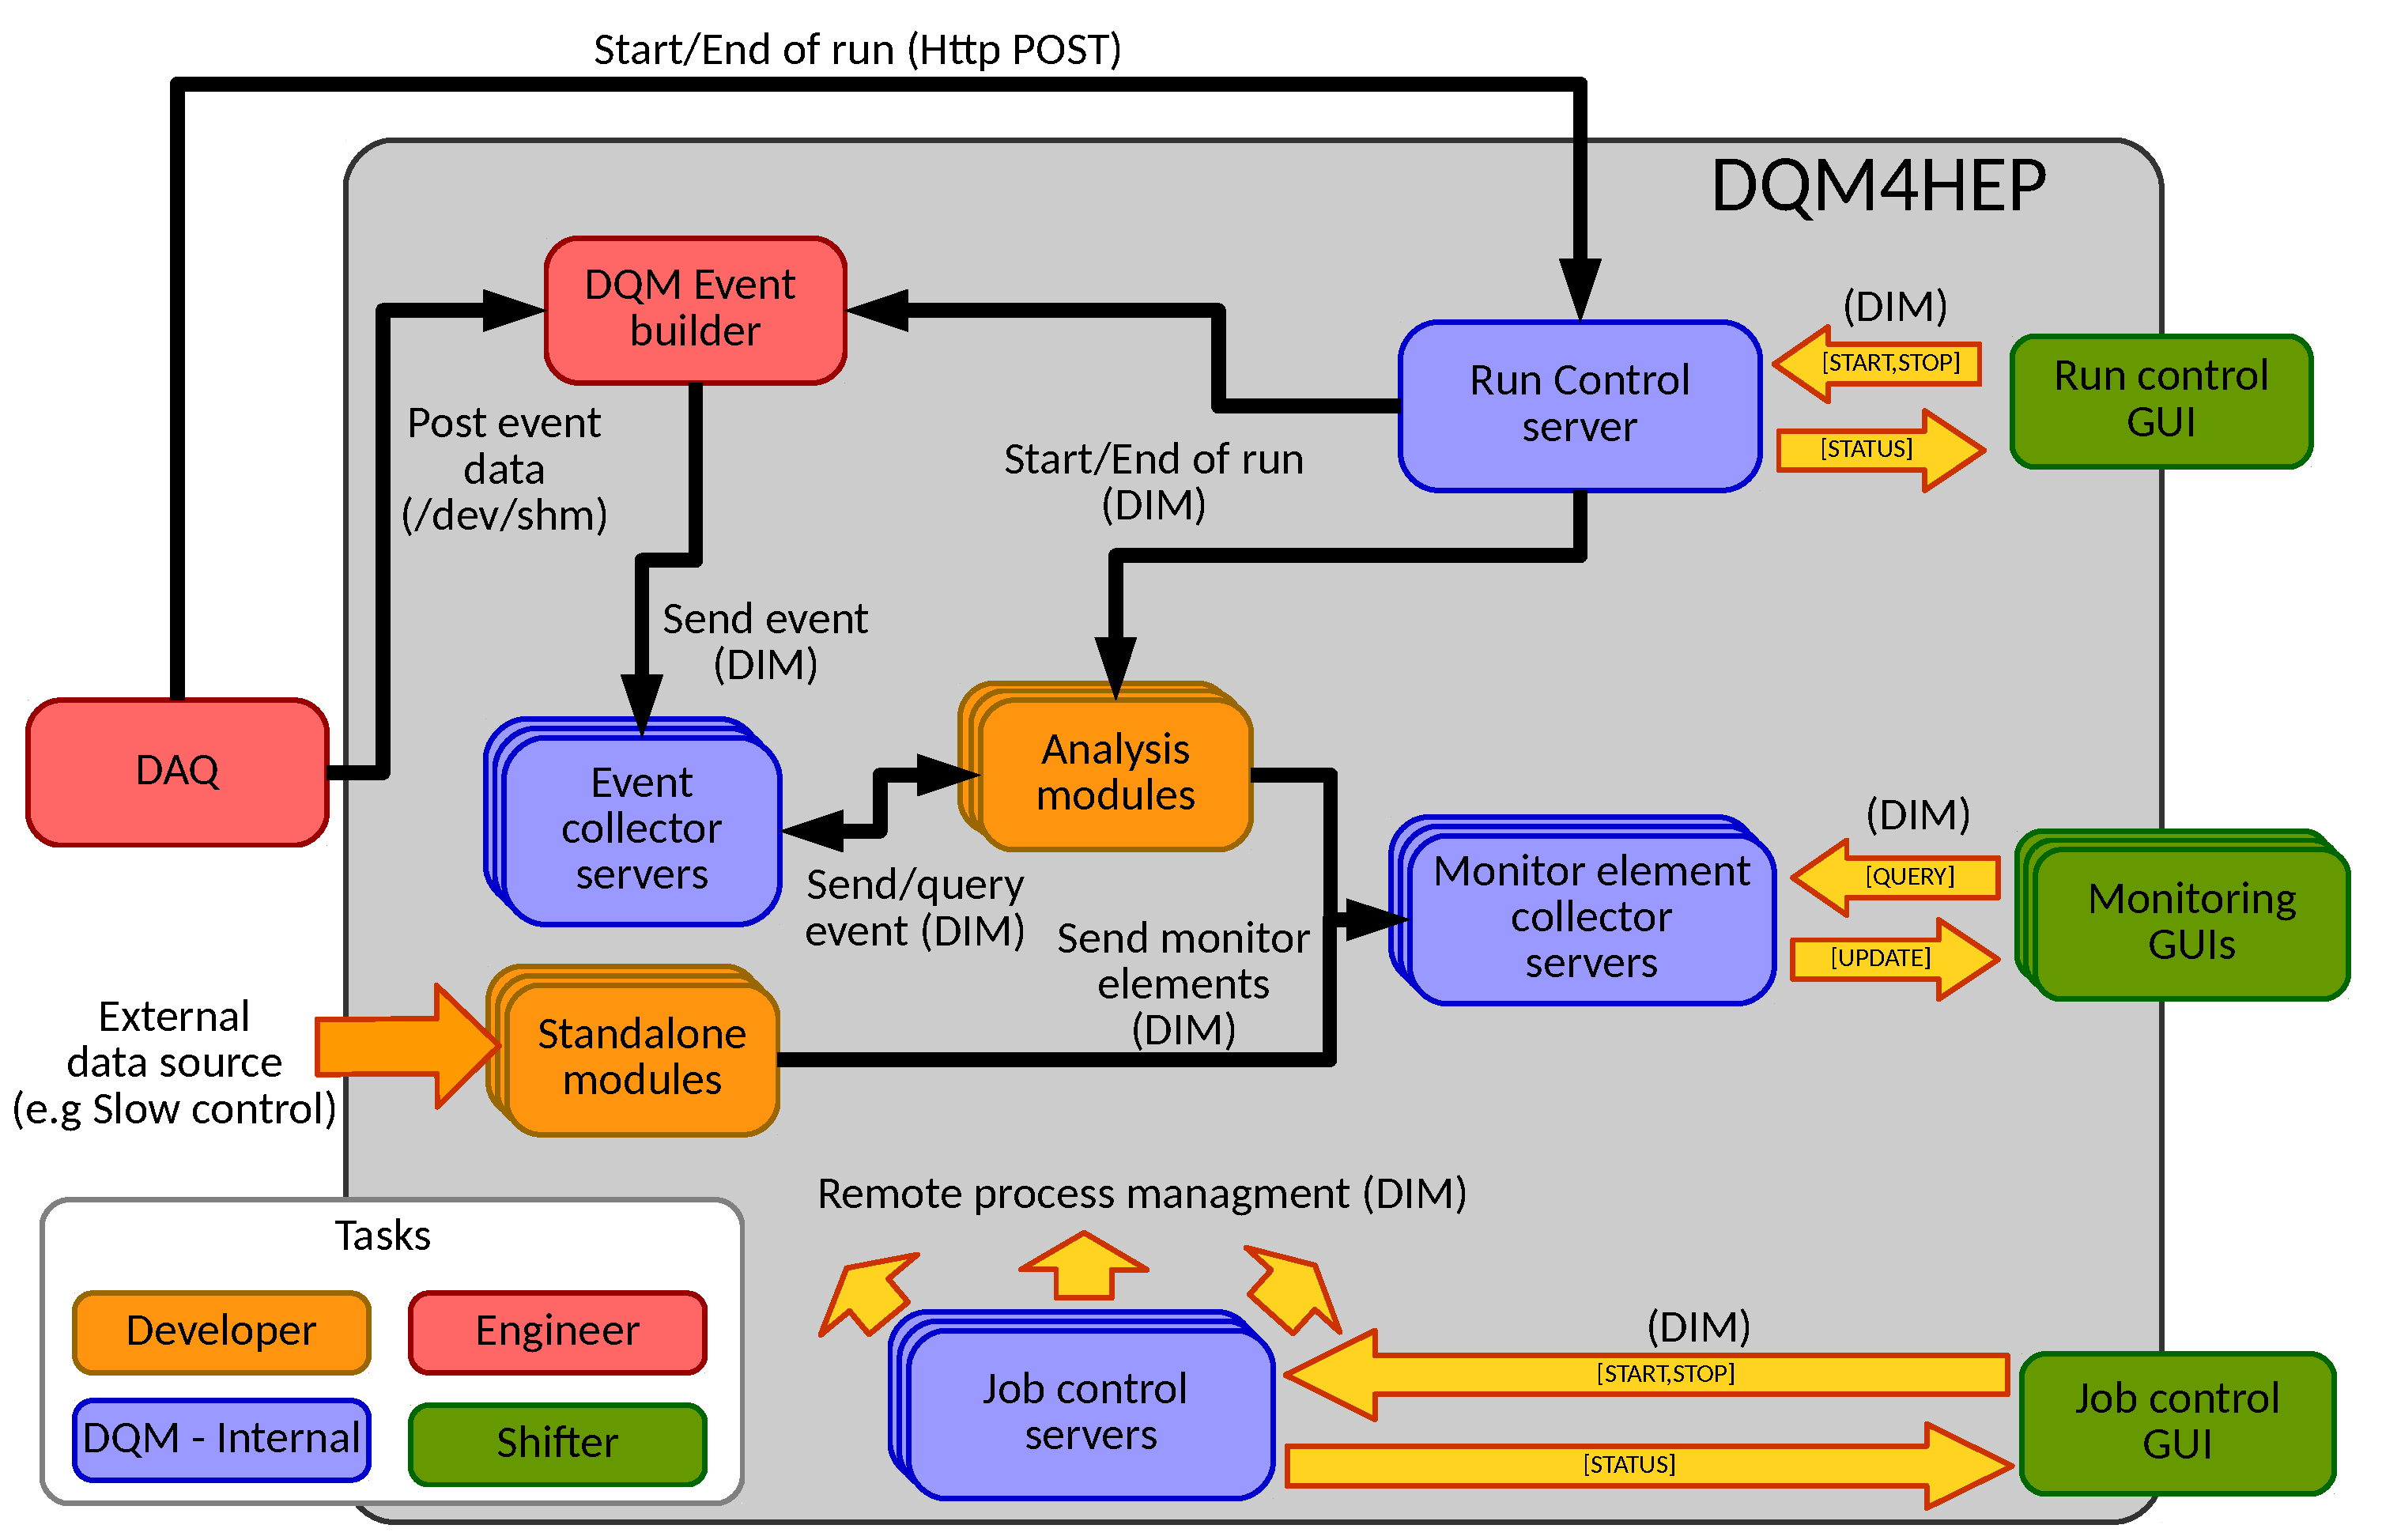
\includegraphics[width=0.9\linewidth]{figs/GlobalArchitectureDiagram.pdf}
\end{frame}

%----------------------------------------------------------------------
\begin{frame}
  \frametitle{DQM4HEP}
  \framesubtitle{Online monitoring interface (Qt Gui)}
    \centering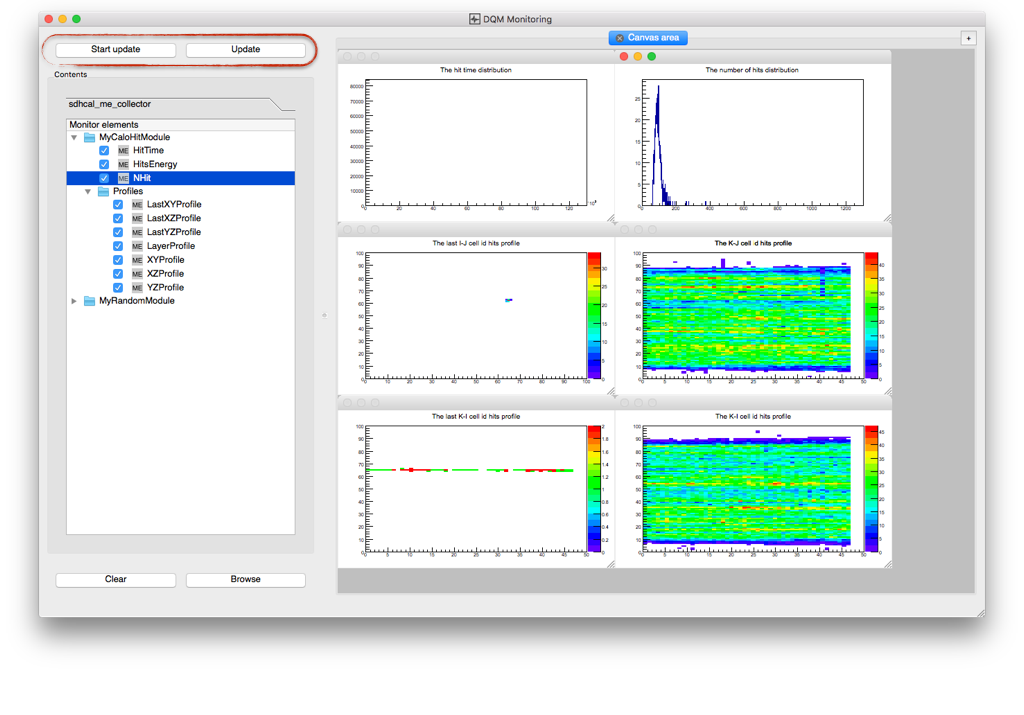
\includegraphics[width=0.95\linewidth]{figs/DQM4HEPMonitoringGui.png}
\end{frame}

\end{document}

% Enable spell checker for vim
% setlocal spell spelllang=en
